\documentclass[12pt,a4paper]{article}
\usepackage[utf8]{inputenc}
\usepackage[brazil]{babel}
\usepackage{graphicx}
\usepackage{amssymb, amsfonts, amsmath}
\usepackage{float}
\usepackage{enumerate}
\usepackage[top=1.5cm, bottom=1.5cm, left=1.25cm, right=1.25cm]{geometry}

\begin{document}
\pagestyle{empty}

\begin{center}
  \begin{tabular}{ccc}
    \begin{tabular}{c}
      \includegraphics[scale=0.25]{../../biblioteca/imagem/brasao-de-armas-brasil} \\
    \end{tabular} & 
    \begin{tabular}{c}
      Ministério da Educação \\
      Universidade Federal dos Vales do Jequitinhonha e Mucuri \\
      Faculdade de Ciências Sociais, Aplicadas e Exatas - FACSAE \\
      Departamento de Ciências Exatas - DCEX \\
      Disciplina: Matemática Elementar I \quad Semestre: 2020/2\\
      Prof. Me. Luiz C. M. de Aquino\\
    \end{tabular} &
    \begin{tabular}{c}
      \includegraphics[scale=0.25]{../../biblioteca/imagem/logo-ufvjm} \\
    \end{tabular}
  \end{tabular}
\end{center}

\begin{center}
 \textbf{Avaliação III}
\end{center}

\textbf{Instruções}
\begin{itemize}
 \item Todas as justificativas necessárias na solução de cada questão devem estar presentes nesta avaliação;
 \item As respostas finais de cada questão devem estar escritas de caneta;
 \item Esta avaliação tem um total de 35,0 pontos.
\end{itemize}

\begin{enumerate}
  \item \textbf{[7,0 pontos]} Os gráficos das funções $f$ e $g$ estão ilustrados abaixo. Determine o ponto de interseção entre esses gráficos.
  
    \begin{figure}[H]
     \centering
     \includegraphics[scale=0.6]{figura/grafico-lista-v-20.2.png}
    \end{figure}
  
  \item \textbf{[7,0 pontos]} Determine os pontos de interseção entre os gráficos das funções definidas por 
  $f(x) = 2x^2 + 10x - 8$ e $g(x) = 5x + 4$.
  
  \item \textbf{[7,0 pontos]} Uma empresa aluga veículos cobrando uma taxa fixa de R\$ 126,00 e mais
    R\$ 15,30 por quilômetro percorrido. Sabendo-se que uma pessoa pagou
    R\$ 11.601,00 após um aluguel nessa empresa, quantos quilômetros essa pessoa
    percorreu com o veículo alugado?

  \item \textbf{[7,0 pontos]} Considere que $f$ é uma função polinomial do 2° grau, cujo o gráfico está
  ilustrado abaixo. Determine os pontos que esse gráfico corta o eixo $x$.

  \begin{figure}[H]
   \centering
   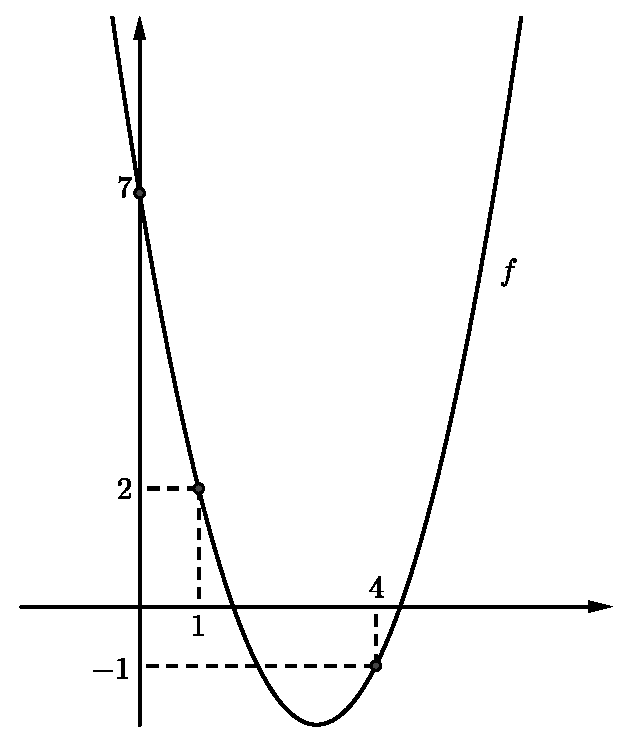
\includegraphics[scale=0.625]{figura/grafico-funcao-polinomio-segundo-grau.eps}
  \end{figure}
  
  \item \textbf{[7,0 pontos]} Determine a expressão da função $f$ polinomial do 2° grau sabendo que seu gráfico 
  corta o eixo $y$ no ponto $(0,\, 6)$, corta o eixo $x$ no ponto $(-2,\, 0)$ e passa
  pelo ponto $(1,\, 8)$.

\end{enumerate}

\end{document}